\section{Statistics for Kociamba's Optimal Solver}
\label{app:kociembaTime}
In order to calculate the time used to solve a \rubik{} using Kociemba's optimal solver, we have gathered data from our application in form of time stamps when ever the solver has finished a search depth.

%The data was gathered on a 2.5 GHz Intel Duo Core processor (P9500) with 4 GB RAM running on Linux-Ubuntu v. 10.04.
The data was gathered on a 2.5 GHz AMD Quad Core processor (905e) with 4 GB DDR-3 RAM running on Windows 7 64 bits.
The data gathered with these specifications are shown in table \ref{tab:timeData} and \ref{tab:timeData2}.

\subsection{First Phase}

\begin{table}[hb]
\centering
	\begin{tabular}{|l|l|l|}
	\hline
	Search depth&First run [ms]&Second run [ms]\\
	\hline
	0&0&0\\
	\hline
	1&0&16\\
	\hline
	2&0&31\\
	\hline
	3&47&78\\
	\hline
	4&281&296\\
	\hline
	5&1045&983\\
	\hline
	6&10920&10873\\
	\hline
	7&157451&158637\\
	\hline
	8&2358584&2361704\\
	\hline
	9&----&35447427\\
	\hline
	\end{tabular}
\caption{\myCaption{Data for computation time to finish a depth in \m{S} of Kociemba's optimal solver, phase one}}
	\label{tab:timeData}
\end{table}

To make the approximation we assume that the time will evolve exponentially based on figure \ref{fig:timeFunction}.

\begin{figure}[tbh]
	\centering
		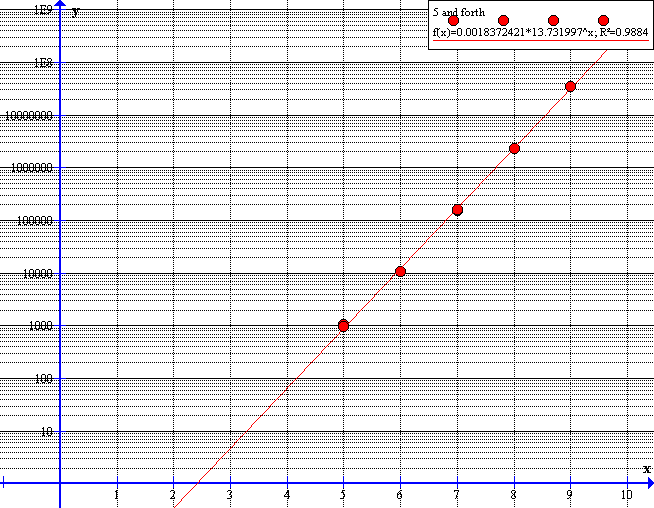
\includegraphics[scale=0.5]{input/pics/timeFunction}
	\caption{\myCaption{The approximation of the time needed to finish the search depth. It is displayed on a logarithmic y-axis to show that an exponential function seem to fit.}}
	\label{fig:timeFunction}
\end{figure}

The figure shows the last four data points since the first five are inaccurate due to small amount time which means that other processes might have interferred with the computation time.

As figure \ref{fig:timeFunction} shows the function for calculating the time needed to finish the search depth $x$ is:
\[
f(x)=0.0035413937 \cdot 13.575029^{x} ms
\]
The $R^2$ is close to 1 and this tell us that the approximation is relatively good. The $R^2$ value is a way to express how well a set of data fits onto a specific approximation -- the closer to 1, the better. We are only interested in a rough approximation on how long the solver needs to use to solve a \rubik{}, therefore our $R^2$ value is very acceptable.

We are interested in approximating the time that it would take to solve a \rubik{}. Since the average \rubik{} needs 18 moves to solve \cite{kociemba09} we will estimate the time to compute this:
\[
f(18) = 0.0035413937 \cdot 13.575029^{18} \approx 8.6798 \cdot 10^{17} ms \approx 27523465 years
\]

After this time our implementation will have solved an average scrambled \rubik{} with the optimal solution.
However the solver will get into \m{H} a long time before this.
As Michael Reid proved in 1995 it takes maximum 12 \twist{}s for Kociemba's optimal solver to enter \m{H}

\subsection{Second Phase}

\begin{table}[hb]
\centering
	\begin{tabular}{|l|l|l|}
	\hline
	Search depth&First run [ms]&Second run [ms]\\
	\hline
	0&2&\\
	\hline
	1&4&\\
	\hline
	2&14&\\
	\hline
	3&74&\\
	\hline
	4&432&\\
	\hline
	5&1775&\\
	\hline
	6&19921&\\
	\hline
	7&289744&\\
	\hline
	8&4339435&\\
	\hline
	9&xxx&xxx\\
	\hline
	10&xxx&xxx\\
	\hline
	11&xxx&xxx\\
	\hline
	12&xxx&xxx\\
	\hline
	\end{tabular}
\caption{\myCaption{Data for computation time to finish a depth in \m{A} of Kociemba's optimal solver, phase two}}
	\label{tab:timeData2}
\end{table}